% !TEX encoding = UTF-8 Unicode
\documentclass[11pt, a4paper, oneside]{article}
\usepackage[onehalfspacing]{setspace}		% One half spacing
\usepackage{hyperref}					% Hyperlinks on pdf (Should be called before Geometry)
\usepackage[a4paper, 					% Page Layout
                     %showframe,				% This shows the frame
                     twoside, includehead,
                     footskip=7mm, headsep=6mm, headheight=4.8mm,
                     marginparsep=2mm, marginparwidth=22mm,
                     top=25mm, bottom=25mm, inner=30mm, outer=25mm]{geometry}
\usepackage{sansmathfonts}				% Sans Serif equations
\usepackage[T1]{fontenc}					% Output font encoding for international characters
\usepackage[utf8]{inputenc}				% Encoding of files: utf8
\renewcommand*\familydefault{\sfdefault} 		% Sans Serif as default font
\usepackage[table]{xcolor}
\usepackage{graphicx}
\usepackage{pdfpages}
\usepackage{array}
\hypersetup{
    colorlinks=true,
    linkcolor=blue,
    filecolor=magenta,      
    urlcolor=blue,
}
\urlstyle{same}
\usepackage{tikz}
\RequirePackage{caption} 				% Caption customization
\captionsetup{justification=centerlast,font=small,labelfont=sc,margin=1cm}

\usepackage{array}
\newcommand{\PreserveBackslash}[1]{\let\temp=\\#1\let\\=\temp}
\newcolumntype{C}[1]{>{\PreserveBackslash\centering}p{#1}}
\newcolumntype{R}[1]{>{\PreserveBackslash\raggedleft}p{#1}}
\newcolumntype{L}[1]{>{\PreserveBackslash\raggedright}p{#1}}

\begin{document}
\begin{titlepage}
	\onehalfspacing
	\enlargethispage{0.65\baselineskip}
	\begin{tikzpicture}[remember picture, overlay]
		\coordinate (top_right) at 
		    ([xshift=-2.5cm, yshift=-2.5cm]current page.north east);
		\coordinate (top_left) at 
		    ([xshift=2.3cm, yshift=-1.8cm]current page.north west);
		\coordinate (bottom_right) at 
		    ([xshift=-1.8cm, yshift=1.8cm]current page.south east);
		\node[inner sep=0, anchor=north east] at (top_right) {\href{http://www.itba.edu.ar}{
\includegraphics[height=19mm, trim={180 200 200 200}, clip]{figs/logo_itba.png}}};
		\draw[double, line width = 0.5pt] (top_left) rectangle (bottom_right);
	\end{tikzpicture}
	\par
	\vspace{-0.8cm}
	\noindent \textbf{CENTRO DE INVESTIGACIÓN Y DESARROLLO EN}\par
	\noindent \textbf{ELECTRONICA INDUSTRIAL (CIDEI)}\par
	\vspace{3cm}
	\begin{center}
		{\Huge \textbf{ARiCE Plattform}\par}
		{\huge \textbf{Getting Started Apio}\par}
	\end{center}
	\vspace{1cm}
	\begin{center}
		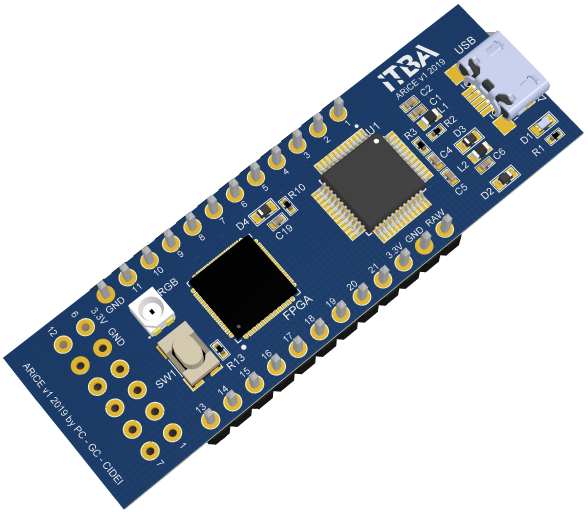
\includegraphics[width=8cm]{figs/fig1a.png}
	\end{center}
	\vfill
	\noindent \textbf{AUTHORS:} Dr. Ing. Pablo \textsc{Cossutta} - Ing. Gonzalo \textsc{Castelli} - Rodrigo \textsc{Devesa} \par
	\vfill
	\begin{center}
		\textbf{CIUDAD AUTÓNOMA DE BUENOS AIRES}\\
		\textbf{2018-2019}\par
	\end{center}
\end{titlepage}

\tableofcontents
\newpage

\section{Introduction}
This project is an open-source platform,shown on Fig. \ref{fig1},  based on a low cost and low consumption FPGA chip from \href{http://www.latticesemi.com}{Lattice Semiconductor}, aiming to be used in a wide range of signal processing and control applications, both for education and the industry.
%
\begin{figure}[h!]
	\centering
	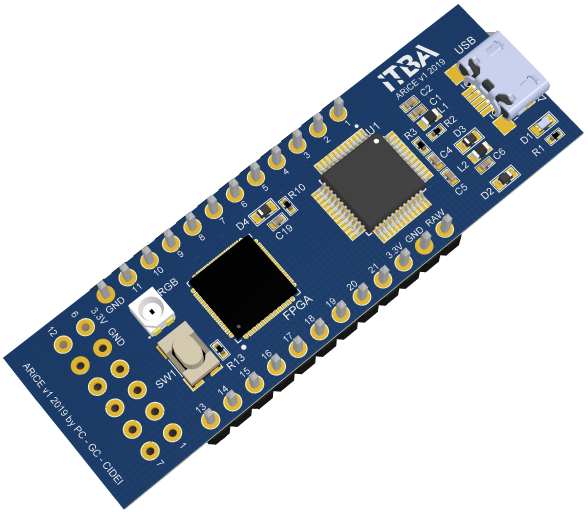
\includegraphics[width=8cm]{figs/fig1a.png}\\
	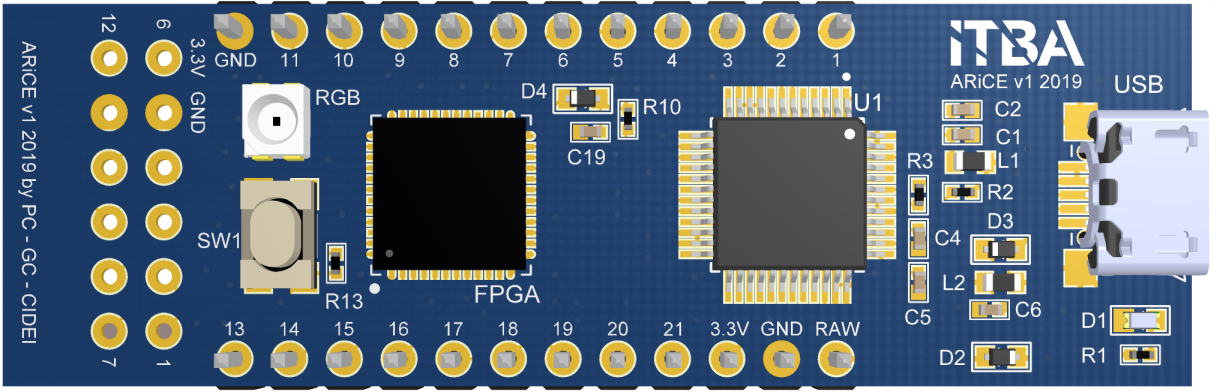
\includegraphics[width=6cm]{figs/fig1b.png}%
	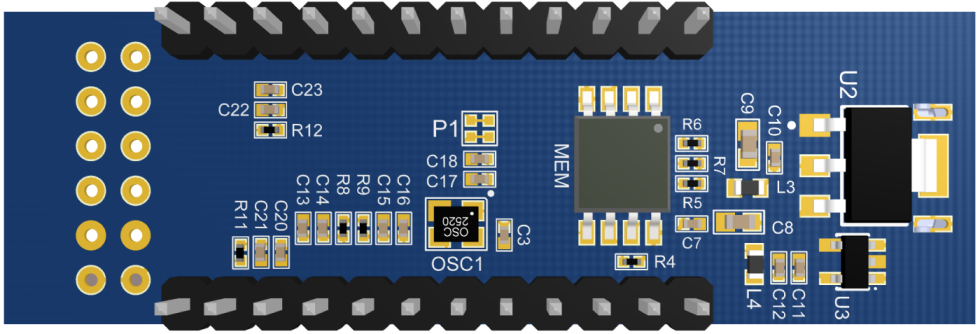
\includegraphics[width=6cm]{figs/fig1c.png}
	\caption{Board's view}
	\label{fig1}
\end{figure}

%\subsection{Project file sources}
%The following list shows the different file sources for this project:
%\begin{itemize}
%	\item Getting Started Guide and Documentation: \href{https://github.com/pcossutta/Lattice-FPGA/tree/master/Documents/Manuals}{GitHub manuals}
%	\item PCB and Schematics: \href{https://workspace.circuitmaker.com/Projects/Details/Gonzalo-Castelli/FPGA-ITBA}{Circuit Maker} and \href{https://github.com/pcossutta/Lattice-FPGA/tree/master/Altium}{GitHub Altium Project Files}
%	\item \href{https://github.com/pcossutta/Lattice-FPGA/tree/master/Examples/LedExample}{Example code} for the Lattice Radiant software.
%\end{itemize}

\section{Getting started}
Without no previous knowledge, three main steps are necessary to use the board if you are starting from scratch. The first is to download and install the software, the second is to create a new project and include the code files needed and finally load the program to the onboard memory using a USB cable.

\subsection{Downloading the software}
Before using the board, it is necessary to set up the software to program the Lattice iCE40-UP5K FPGA chip. In this tutorial we will be utilizing the  \href{https://apiodoc.readthedocs.io/en/stable/index.html}{Apio Open Source Ecosystem for FPGAs}, which allows to verify the code and program the FPGA through a USB port.\href{https://apiodoc.readthedocs.io/en/stable/index.html}{Python 3.7+} should be previously installed in order to install Apio.

During Python installation, make sure to select "\textbf{Customize Installation}". Then, on the optional features screen, select to install pip, as shown in  Fig. \ref{fig2}, as we will be using it to download the Apio packages.
\ref{fig2}.

\begin{figure}[h!]
    \centering
    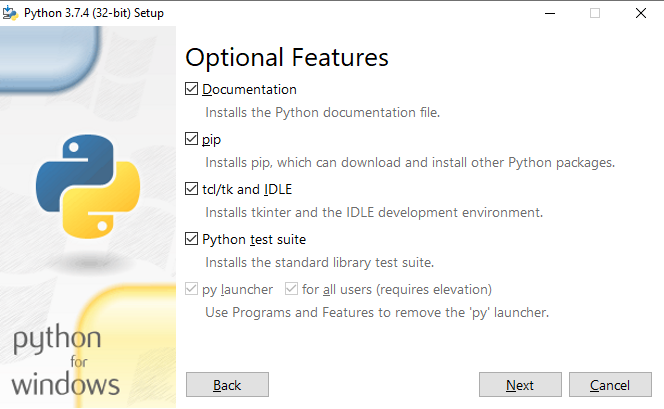
\includegraphics[width=0.8\textwidth]{figs/python_install.png}
    \caption{Setting up the Python installation}
    \label{fig2}
\end{figure}

Once Python is successfully installed along with Pip, you can install Apio. On Windows, open your command line console and type:
\begin{center}
	\texttt{pip install -U apio}
\end{center}
When it's finished, you will need to install Apio's packages. Use the following command:
\begin{center}
	\texttt{apio install -{}-all}
\end{center}
This installation might take a few minutes.

\subsection{Creating a new project}
After having installed the software, the next step is to create a new folder for the project and start writing the code. An example code that uses the onboard RGB LED is available for download at the GitHub repository of this project. After downloading the files, place them in an easily accessible folder from where we will run the code.

Use the \texttt{cd} command followed by the path to your project's folder to change directory to that folder. For example, if your project is on a folder called "fpga\_project" in your Desktop, then use:
\begin{center}
	\texttt{cd Desktop/fpga\_project}
\end{center}

Once in the right folder, you need to generate the right .init configuration file for this board, as Apio supports multiple different FPGA platforms. To do this, use the command:

\begin{center}
	\texttt{apio init -{}-board upduino2}
\end{center}

Now, to make sure the project is set up correctly, you could use the command:
\begin{center}
	\texttt{apio build}
\end{center}
The folder should contain at least 3 files, one .v file with the program's code itself, one .pcf file with pinout information for the program, and the .init file we just created. If the build process is successful, you can move on to programming the FPGA board.
 
\subsection{Programming the board}
Now that the project is fully set up, we can load the program into our board to run it.
Connect the FPGA board to the PC using the USB cable, wait a few seconds for Windows to configure the drivers, then use the following command to program the board:
\begin{center}
	\texttt{apio upload}
\end{center}
The process will take a few seconds, and if everything went right, the FPGA board should start running the program and its onboard LED should start flashing in colors.

\subsection{Model simulation}
To simulate the model the following command is used:
\begin{center}
	\texttt{apio sim}
\end{center}

The \href{http://gtkwave.sourceforge.net}{GTKWave} graphic environment should be load with the simulation data.
% !TEX encoding = UTF-8 Unicode
\newpage
\section{Pinout information}
The board has multiple I/O pins, as well as power supply pins, distributed along the side and the front of the PCB. The next list gives a short description of the signals:
\begin{itemize}
	\item IOT\_XX are general I/O pins. In user mode, after configuration, these pins can be programmed as I/O in user function in the top (xx = I/O location)
	\item IOB\_XX are general I/O pins. In user mode, after configuration, these pins can be programmed as I/O in user function in the bottom (xx = I/O location)
	\item RAW VCC. The input voltage to the FPGA board when it's using an external power source. The board can be supplied with power either from the USB connector or the RAW VCC pin. The nominal supply voltage is 5V. (Minimum is 4.5V and maximum is 6V)
	\item 3.3V. A 3.3 volt supply generated by the on-board regulator. Maximum recommended current draw from this pin is 500 mA
	\item GND. Ground pins
	\item Signal names with G1, G3 and G6 suffixes may be used as a General I/O or as a Global input used for high fanout, or clock/reset net. These pins drive the GBUF1, GBUF3 and GBUF6 global buffers respectively
\end{itemize}

\newpage
Table \ref{table1} shows the mapping between the signals and the board pin numbers.
\definecolor{myHdr}{rgb}{0.81000,0.8800,0.9400}%
\begin{table}[h!]
	\renewcommand{\arraystretch}{1.3}
	\caption{Connections}
	\label{table1}
	\begin{tabular}[t]{C{0.12\textwidth} C{0.12\textwidth} C{0.15\textwidth}}
		\bfseries Board Pin & \bfseries FPGA Pin & \bfseries Signal Name \\ \hline
		\rowcolor{myHdr} \multicolumn{3}{c}{\bfseries Side Pins} \\ \hline
		1 & 20 & IOB 25B G3 \\
		2 & 21 & IOB 23B \\
		3 & 23 & IOT 37A \\
		4 & 25 & IOT 36B \\
		5 & 26 & IOT 39A \\
		6 & 27 & IOT 38B \\
		7 & 31 & IOT 42B \\
		8 & 32 & IOT 43A \\
		9 & 34 & IOT 44B \\
		10 & 36 & IOT 48B \\
		11 & 37 & IOT 45A G1 \\
		12 & - & GND \\
		& & \\
		13 & 2 & IOB 6A \\
		14 & 6 & IOB 13B \\
		15 & 9 & IOB 16A \\
		16 & 10 & IOB 18A \\
		17 & 11 & IOB 20A \\
		18 & 12 & IOB 22A \\
		19 & 13 & IOB 24A \\
		20 & 18 & IOB 31B \\
		21 & 19 & IOB 29B \\
		22 & - & 3.3V \\
		23 & - & GND \\
		24 & - & RAW VCC \\
	\end{tabular}
	\quad
	\begin{tabular}[t]{C{0.12\textwidth} C{0.12\textwidth} C{0.15\textwidth}}
		\bfseries Board Pin & \bfseries FPGA Pin & \bfseries Signal Name \\ \hline
		\rowcolor{myHdr} \multicolumn{3}{c}{\bfseries Front Pins} \\ \hline
		1 & 4 & IOB 8A \\
		2 & 3 & IOB 9B \\
		3 & 47 & IOB 2A \\
		4 & 44 & IOB 3B G6 \\
		5 & - & GND \\
		6 & - & 3.3V \\
		7 & 48 & IOB 4A \\
		8 & 45 & IOB 5B \\
		9 & 38 & IOT 50B \\
		10 & 42 & IOT 51A \\
		11 & - & GND \\
		12 & - & 3.3V \\
		& & \\
		\bfseries Board Pin & \bfseries FPGA Pin & \bfseries Signal Name \\ \hline
		\rowcolor{myHdr} \multicolumn{3}{c}{\bfseries Not Connected} \\ \hline
		 - & 43 & IOT 49A \\
		- & 46 & IOB 0A \\
		- & 28 & IOT 41A \\	
		& & \\
		& & \\
		\bfseries LED Color & \bfseries FPGA Pin & \bfseries Signal Name \\ \hline
		\rowcolor{myHdr} \multicolumn{3}{c}{\bfseries Onboard RGB LED} \\   \hline
		Blue & 39 & RGB0 \\
		Green & 40 & RGB1 \\
		Red & 41 & RGB2 \\
	\end{tabular}
\end{table}

\newpage
The differential pairs are shown in Table \ref{table2}. They are grouped together and labeled in colors, white is positive and light blue is negative.
%
\begin{table}[h!]
	\renewcommand{\arraystretch}{1.3}
	\caption{Differential Pairs}
	\vspace{0.5em}
	\label{table2}
	\centering
	\begin{tabular}{C{0.12\textwidth} C{0.12\textwidth} C{0.15\textwidth}}
		\bfseries Board Pin & \bfseries FPGA Pin & \bfseries Signal Name \\ \hline
		\rowcolor{myHdr}  3 & 23 & IOT 37A \\
		4 & 25 & IOT 36B \\ \hline
		\rowcolor{myHdr}  5 & 26 & IOT 39A \\
		6 & 27 & IOT 38B \\ \hline
		\rowcolor{myHdr}  8 & 32 & IOT 43A \\
		7 & 31 & IOT 42B \\ \hline
		\rowcolor{myHdr}  11 & 37 & IOT 45A G1 \\
		9 & 34 & IOT 44B \\ \hline
		\rowcolor{myHdr}  2 & 21 & IOB 23B \\
		18 & 12 & IOB 22A \\ \hline
		\rowcolor{myHdr}  2 & 3 & IOB 9B \\
		1 & 4 & IOB 8A \\ \hline
		\rowcolor{myHdr}  4 & 44 & IOB 3B G6 \\
		3 & 47 & IOB 2A \\ \hline
		\rowcolor{myHdr}  8 & 45 & IOB 5B \\ 
		7 & 48 & IOB 4A \\ \hline
		\rowcolor{myHdr}  10 & 42 & IOT 51A \\ 
		9 & 38 & IOT 50B \\
	\end{tabular}
\end{table}

\section{Open Source PCB}
The board files, circuit schematics and list of components are available in the GitHub repository. Altium project and Gerber files are available. The board is also published in open source EDAs just as \href{https://workspace.circuitmaker.com/}{Circuit Maker} and \href{http://www.kicad-pcb.org}{KiCad}.

\newpage
\subsection{Bill of Materials}
Table \ref{table3} includes all the components in the FPGA Board. Follow the hypertext links to the component's datasheets for further information.
%
\begin{table}[h]
	\renewcommand{\arraystretch}{1.3}
	\caption{Bill of materials}
	\vspace{0.5em}
	\label{table3}
	\centering
	\begin{tabular}{p{4cm} C{0.5cm} c C{1cm} p{2cm}}
		\bfseries Designator & \bfseries Qty & \bfseries Manufacturer Part Number & \bfseries Value & \bfseries Footprint \\ \hline
		C2, C3, C4, C5, C6, C10, C12, C14, C16, C18, C19, C21, C23 & 13 & \href{http://www.samsungsem.com/kr/support/product-search/mlcc/CL05B104KA5NNNC.jsp}{CL05B104KA5NNNC} & 0.1uF & 0402 \\ \hline
		C8, C9 & 2 & \href{http://www.yageo.com/documents/recent/UPY-GPHC_X5R_4V-to-50V_25.pdf}{CC0603KRX5R8BB105} & 1uF & 0603 \\ \hline
		C1, C7, C11, C13, C15, C17, C20, C22 & 8 & \href{https://product.tdk.com/info/en/catalog/datasheets/mlcc_commercial_lowprofile_en.pdf}{CGB2A1JB1E105M033BC} & 1uF & 0402 \\ \hline
		R1 & 1 & \href{http://www.yageo.com/documents/recent/PYu-RC_Group_51_RoHS_L_9.pdf}{RC0402JR-071KL} & 1K$\Omega$ & 0402 \\ \hline
		R2 & 1x& \href{http://www.yageo.com/documents/recent/PYu-RC_Group_51_RoHS_L_9.pdf}{RC0402FR-072K2L} & 2.2k$\Omega$ & 0402 \\ \hline
		R3, R4, R5, R6, R7, R13 & 6 & \href{http://www.yageo.com/NewPortal/yageodocoutput?fileName=/pdf/R-Chip/PYu-RC_51_RoHS_P_0.pdf}{RC0402JR-0710KP} & 10k$\Omega$ & 0402 \\ \hline
		R8, R9, R10, R11, R12 & 5 & \href{http://www.yageo.com/NewPortal/yageodocoutput?fileName=/pdf/R-Chip/PYu-AC_51_RoHS_L_6.pdf}{AC0402JR-071RL} & 1$\Omega$ & 0402 \\ \hline
		L1 & 1 & \href{http://assets.lairdtech.com/home/brandworld/files/HI0603P600R-10.pdf}{HI0603P600R-10} & 10mH & 0603 \\ \hline
		L2, L3, L4 & 3 & \href{https://www.murata.com/en-us/products/productdata/8796741599262/ENFA0004.pdf}{BLM18HE601SN1D} & 10mH & 0603 \\ \hline
		RGB & 1 & \href{https://www.cree.com/led-components/media/documents/1273-CLMVC-FKA.pdf}{CLMVC-FKA-CL1D1L71BB7C3C3} & & 4-PLCC \\ \hline
		D1 & 1 & \href{http://optoelectronics.liteon.com/upload/download/DS-22-99-0224/LTST-C190TBKT.PDF}{LTST-C190TBKT} & & 0603 \\ \hline
		U1 & 1 & \href{http://www.ftdichip.com/Support/Documents/DataSheets/ICs/DS_FT232H.pdf}{FT232HL-REEL} & & 48-LQFP (7x7) \\ \hline    
		U2 & 1 & \href{http://www.ti.com/lit/ds/symlink/tlv1117lv.pdf}{TLV1117LV33DCYR} & & SOT-223-4 \\ \hline
		U3 & 1 & \href{http://www.ti.com/lit/ds/symlink/lp5907.pdf}{LP5907MFX-1.2/NOPB} & & SOT-23-5 \\ \hline
		OSC1 & 1 & \href{https://media.digikey.com/pdf/Data\%20Sheets/SiTime\%20PDFs/SIT1602A.pdf}{SIT1602AC-73-33S-12.000000G} & & 2.0X1-6MM \\ \hline
		FPGA & 1 & \href{http://www.latticesemi.com/view_document?document_id=51968}{ICE40UP5K-SG48ITR50} & & 48-QFN-7X7 \\ \hline
		USB & 1 & \href{http://www.amphenol-icc.com/media/wysiwyg/files/drawing/10118193.pdf}{10118193-0001LF} & & Micro USB B SMD \\ \hline
		MEM & 1 & \href{https://www.winbond.com/resource-files/w25q32jv%20dtr%20revf%2002242017.pdf}{W25Q32JVSSIQ} & & SOP8 \\ \hline
		D2, D3, D4 & 3 & \href{http://www.comchiptech.com/admin/files/product/CDBU0520-HF-RevA797161.pdf}{CDBU0520} & & 0603/SOD-523F \\ \hline
		SW1 & 1 & \href{https://www.ckswitches.com/media/1465/kxt3.pdf}{PTS810 SJM 250 SMTR LFS} & & SW4-SMD \\
	\end{tabular}
\end{table}

\subsection{Schematics}
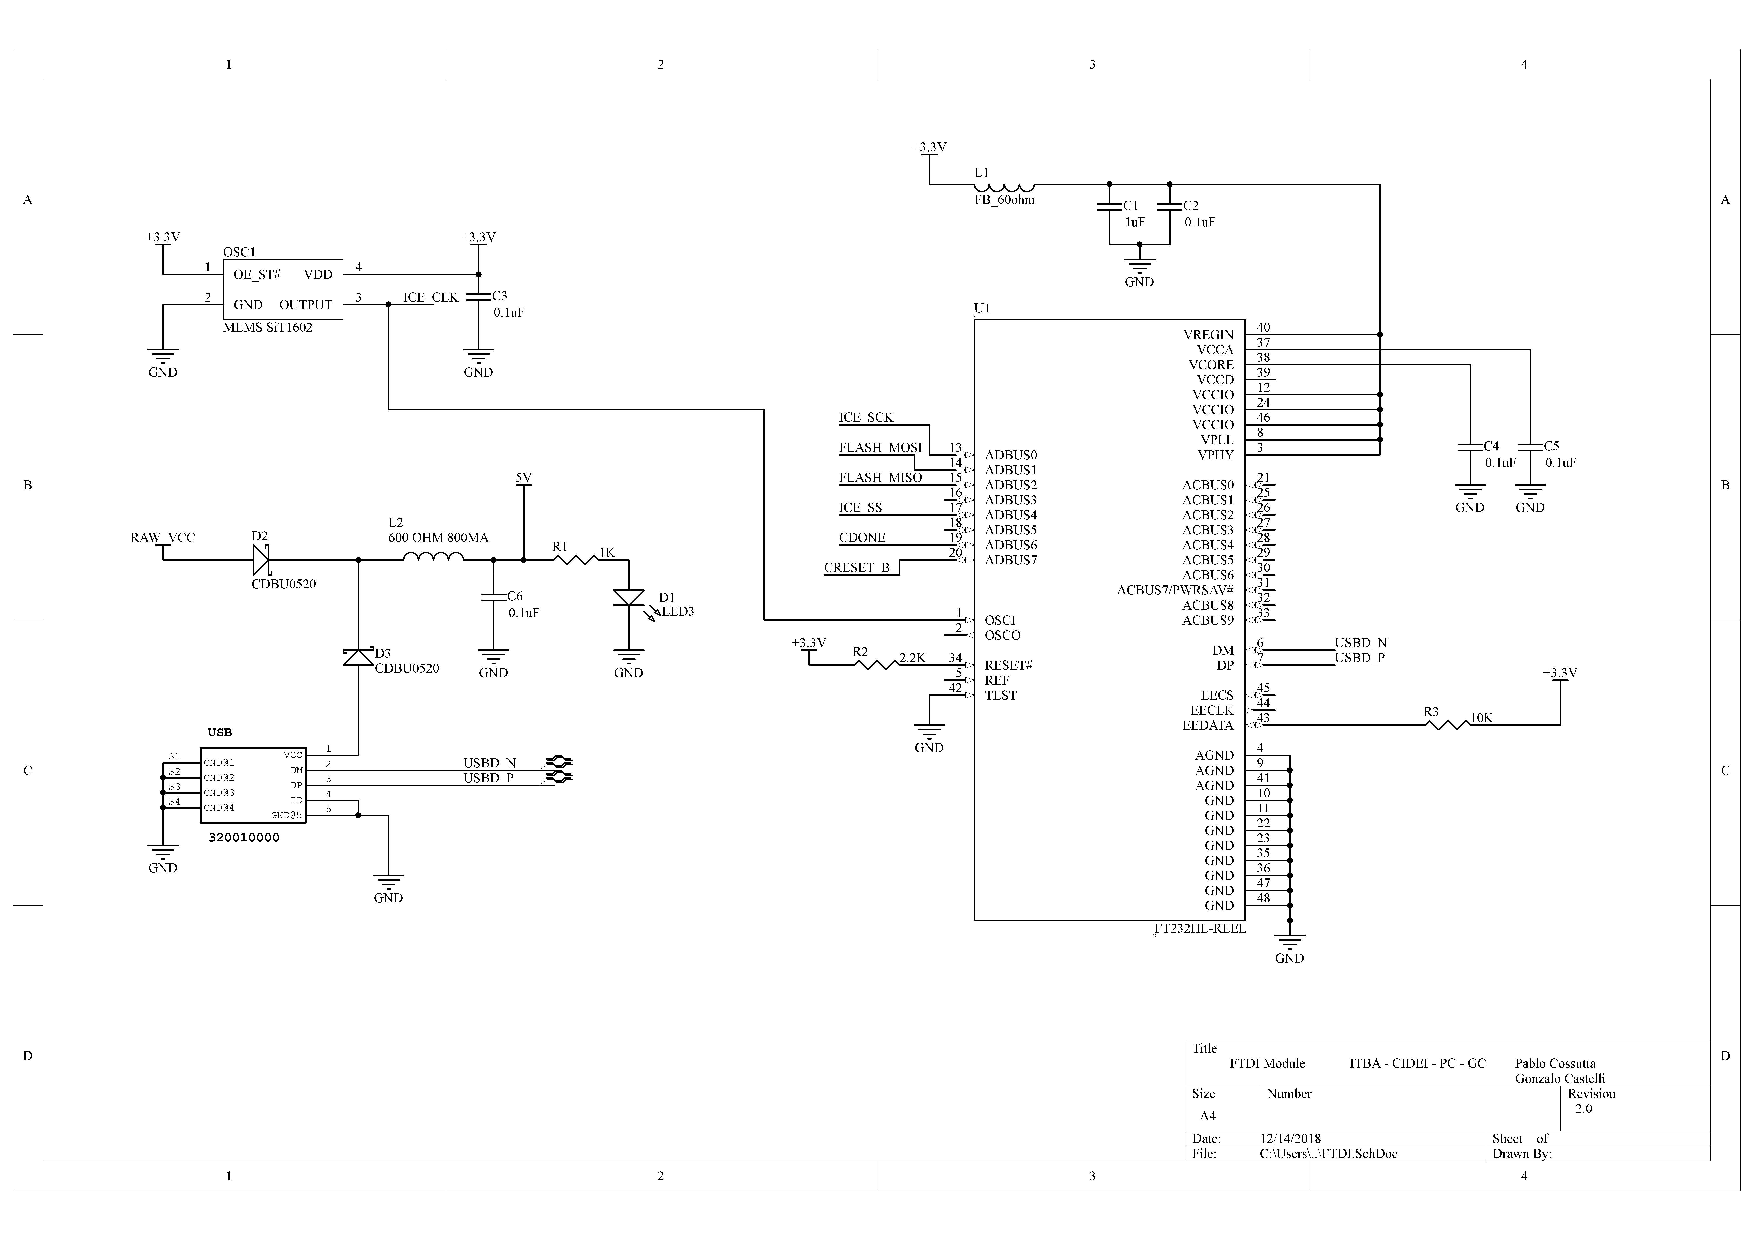
\includepdf[landscape=true]{figs/ftdi.pdf}
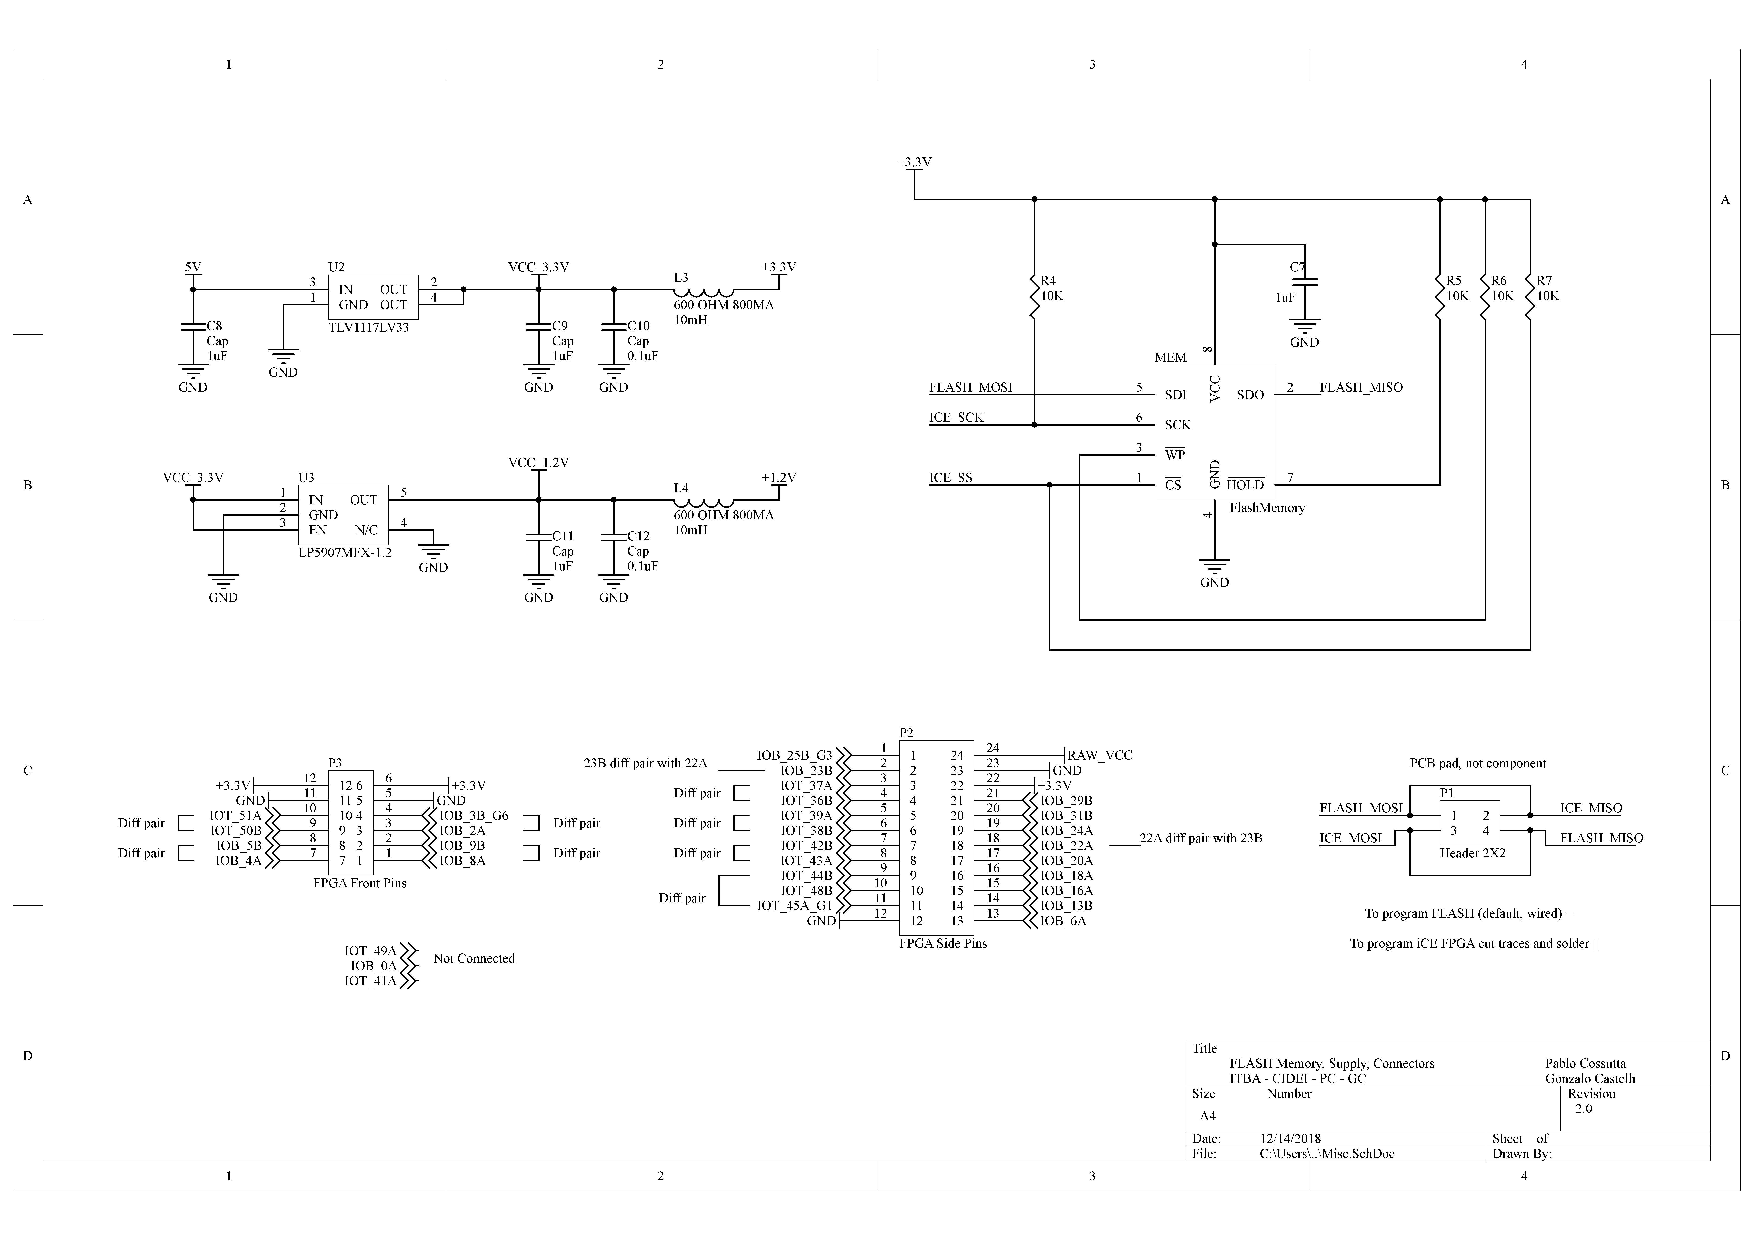
\includepdf[landscape=true]{figs/misc.pdf}
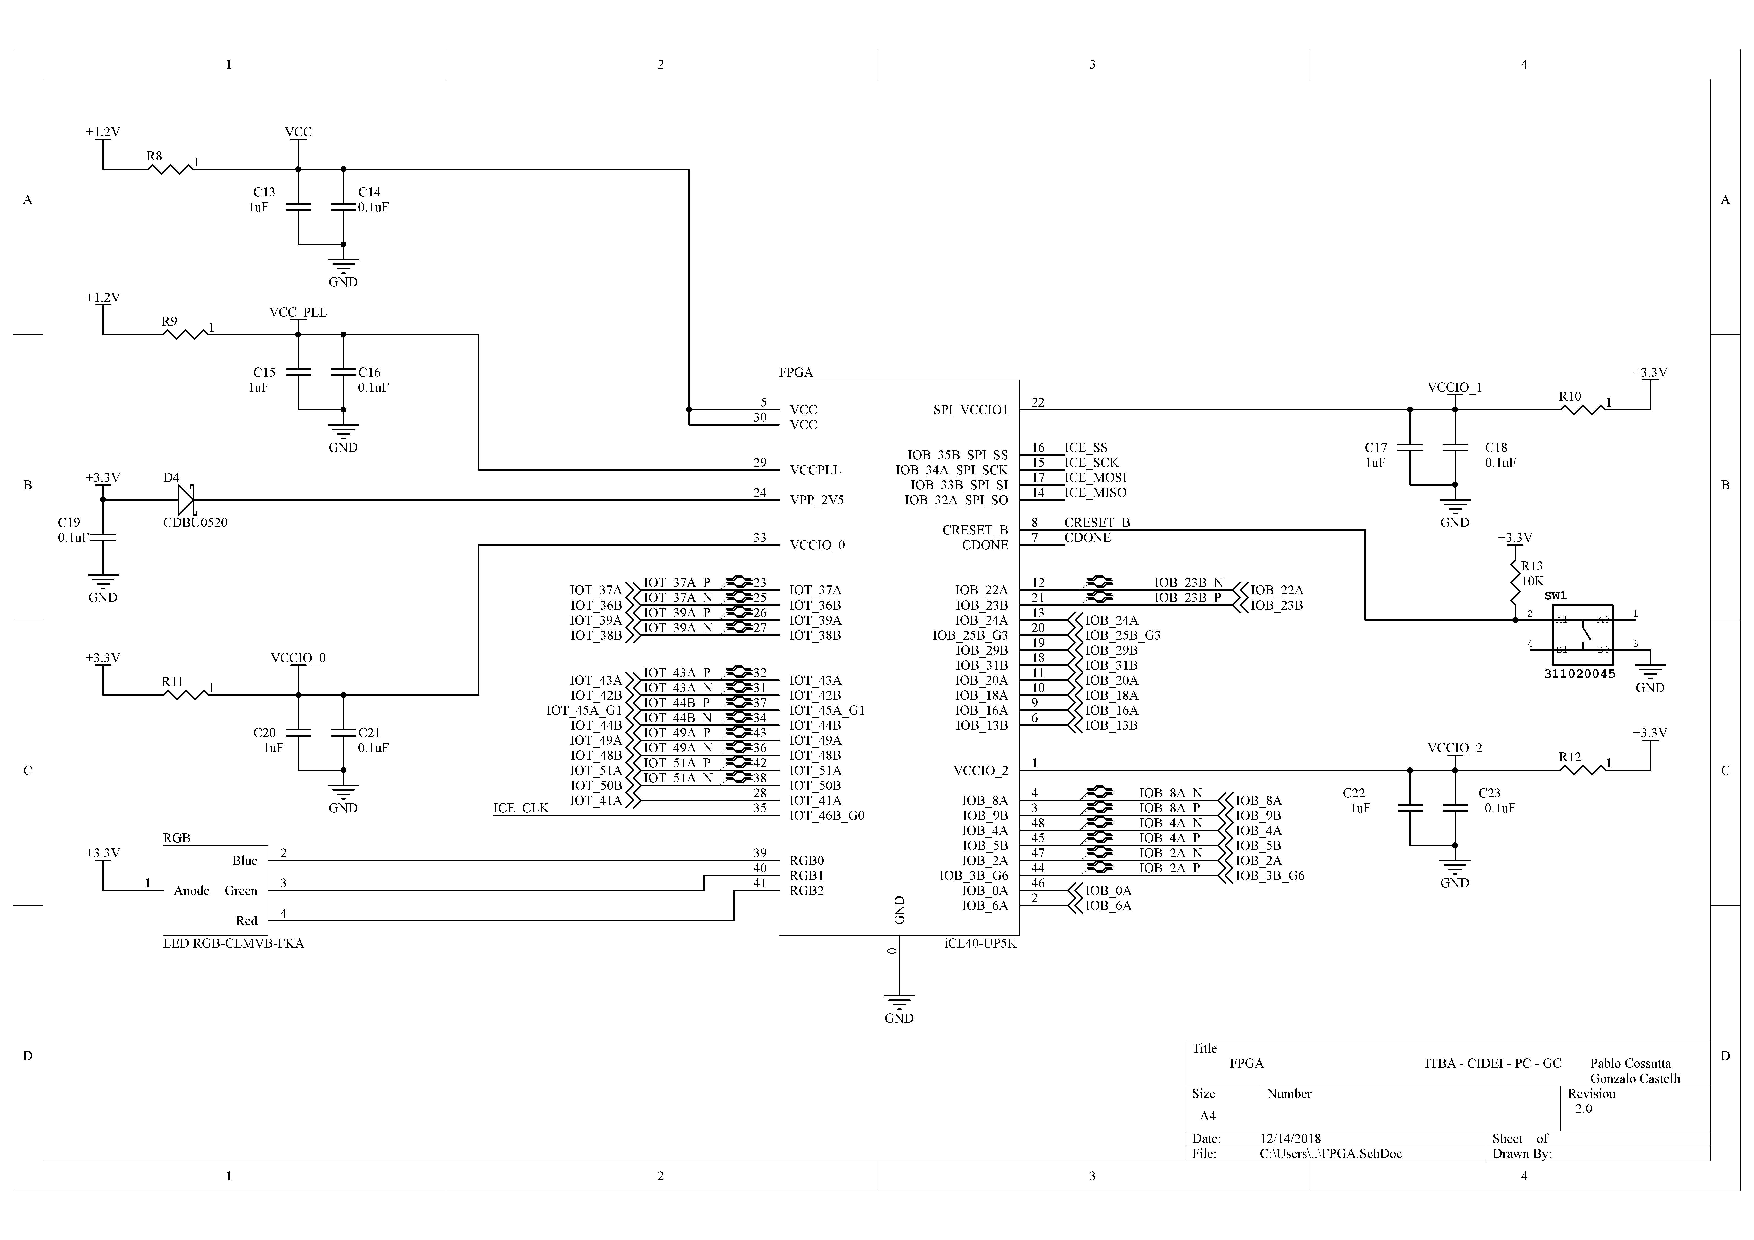
\includepdf[landscape=true]{figs/fpga.pdf}

\section{License}
This project is licensed under a Creative Commons Attribution Share-Alike license, meaning that you are free to use and adapt it for your own needs without asking for permission or paying a fee, even for commercial purposes, as long as you give appropriate credit and release the design under the same license. Visit the
\href{https://creativecommons.org/licenses/by-sa/3.0/}{Creative Commons Website} for further information.

\section{Acknowledgments}
The circuit was inspired by the official manuals and toolchain of the \href{http://www.latticesemi.com/en/Products/DevelopmentBoardsAndKits/iCE40UltraPlusBreakoutBoard.aspx}{iCE40 UltraPlus Breakout Board} from Lattice, and the documentation of the iCE40UP5K FPGA chip.

\end{document}